\documentclass[aspectratio=43,t]{beamer}
%\documentclass[aspectratio=43,t,handout]{beamer}

% Language and General Settings
\usepackage[T1]{fontenc} 				% Umlauts and correct hyphenation
\usepackage[utf8]{inputenc} 			% Unicode t
\usepackage{textcomp} 				% Various symbols (e.g. �, �) 
\usepackage{amsmath}				% Math environment
\usepackage{mathtools}				% Math environment for curly brackets
\usepackage{bm}					% Boldface inside math environment
\usepackage{amssymb} 				% Various mathematical symbols
\usepackage{hyperref} %\usepackage[hidelinks]{hyperref}			% Links within document not labeled
\usepackage[final]{microtype}			% Better justification
\usepackage{color}					% Enables definition of own colors

% Listings
\usepackage{listings} 					% Program code environment
\lstset{
	language=C++, 
	showstringspaces=false,
	breaklines=true,
	basicstyle=\tiny\ttfamily,
	keywordstyle=\color{blue},
	stringstyle=\color{red},
	commentstyle=\color{green},
	morecomment=[l][\color{magenta}]{\#},
	title=\lstname}

% Images/ Plots
\usepackage{pgfplots}					% Enables including of tikz-images
\usetikzlibrary{calc}
\pgfplotsset{compat=newest}%
\pgfplotsset{table/search path ={../}}		% Search path for data is lowest directory now
\newlength\figureheight 				% Command to adjust the size of pgf-plots
\newlength\figurewidth
\usepackage{graphicx}					% Enables including of various graphics formats
\usepackage{caption}					% Enables including of various graphics formats
\usepackage{subcaption}				% Enables subfigures
\usepackage{chngcntr}				% Continuous numbering of images
\usepackage{epstopdf}				% Enables including of eps-images
\graphicspath{img/}					% Path to images
\usepackage{adjustbox}
\usepackage{smartdiagram}
\usepackage{multimedia}

%English version FAU Logo
\usepackage[english]{babel}
%German version FAU Logo
%\usepackage[ngerman]{babel}
\usepackage[backend=biber,sorting=none,doi=true,style=ieee]{biblatex}

% Themes:
%  - fau:          FAU theme
%  - fau-med:      MedFak FAU theme
%  - fau-nat:      NatFak FAU theme
%  - fau-phil:     PhilFak FAU theme
%  - fau-rw:       RWFak FAU theme
%  - fau-rw-jura:  RWFak FB Jura FAU theme
%  - fau-rw-wiso:  RWFak FB WISO FAU theme
%  - fau-tf:       TechFak FAU theme
%
% Options:
%  - image:        Cover image on title page
%  - plain:        Plain title page
%  - longtitle:    Title page layout for long title
\makeatletter
  \def\beamer@calltheme#1#2#3{%
    \def\beamer@themelist{#2}
    \@for\beamer@themename:=\beamer@themelist\do
    {\usepackage[{#1}]{\beamer@themelocation/#3\beamer@themename}}}

  \def\usefolder#1{
    \def\beamer@themelocation{#1}
  }
  \def\beamer@themelocation{}

\usefolder{themefau}
\usetheme[longtitle]{fau-tf}

% Enable semi-transparent animation preview
\setbeamercovered{transparent}

\defbibheading{bibliography}{}
\addbibresource[label=primary]{../literature.bib}

\usepackage{csquotes}																% Avoids warning when using BibLaTeX
\usepackage[noabbrev]{cleveref}																% Have automatic formatting of references: use \cref or \Cref{labellist} instead of \ref 
%\crefname{section}{}{}
\usepackage{siunitx}														% format SI units
\usepackage{smartdiagram}

% Title, authors, and date
\title[Comparison between LBM and FEM for Earth Mantle Simulation]{Comparison between Lattice Boltzmann Methods and Finite Elements for Earth Mantle Simulation}
\subtitle{BGCE Honours Project}
\author[T. Pollinger, C. Schwarzmeier, N. Dommaraju]{Theresa Pollinger, Christoph Schwarzmeier, Nivesh Dommaraju}
% English version
\institute[LSS]{Chair for System Simulation, Friedrich-Alexander University of Erlangen-Nuremberg}
% German version
%\institute[Lehrstuhl f\"ur XYZ]{Lehrstuhl f\"ur XYZ, Friedrich-Alexander-Universit\"at Erlangen-N\"urnberg}
\date{\today}
% Set additional logo (overwrites FAU seal)

% Setting right internal properties for the pdf-file
\usepackage{ifpdf}
\ifpdf
\hypersetup{pdfauthor={Theresa Pollinger, Christoph Schwarzmeier, Nivesh Dommaraju}}
\hypersetup{pdftitle={Comparison between Lattice Boltzmann Methods and Finite Elements for Earth Mantle Simulation}}
\fi

\begin{document}
 

% Title
\maketitle


  { % Outline
    \setbeamertemplate{footline}{}
    \begin{frame}[noframenumbering]{Outline}
      \tableofcontents
    \end{frame}
  }
  
\section{Introduction}

\begin{frame}{Earth Mantle Convection II}
\begin{itemize}
	\item Creeping flow, according to \cite{weismueller.2015}:
		\begin{align*}
		\begin{rcases}
		\mu &\approx10^{21}\,\text{Pa}\cdot \text{s}\\
		u &\approx3\,\text{cm/a}\\
		h &=2 867\,\text{km}\\
		\rho &\approx4000\,\text{kg/m}^3
		\end{rcases}
		Re =\frac{\rho \cdot u \cdot h}{\mu}\approx10^{-20} \ll 1
		\end{align*}
\pause
	\item Dominant viscous forces, negligible intertial forces
	\item \textit{Navier-Stokes} equations simplify to \textit{Stokes} equations
		\begin{align*}
		\mu\Delta \bm{u}-\nabla p + \bm{f} &= \bm{0}\\
		\nabla \cdot \bm{u} &= \bm{0}
		\end{align*}
\end{itemize}

\end{frame}

\begin{frame}{Derivation of a Benchmark II}
\begin{itemize}
\item[]
	\begin{itemize}
		\item Construct a divergence-free velocity field
			\begin{align*}
				\begin{bmatrix}
				u\\
				v
				\end{bmatrix}
				=\nabla^\perp\Phi=
				\begin{bmatrix}
				\sin(2\pi x)\cos(\pi y)\\
				-2\cos(2\pi x)\sin(\pi y)
				\end{bmatrix}
			\end{align*}
\pause
		\item Construct the pressure field according to the \textit{Stokes} equations with $\mu=1$
			\begin{align*}
				\bm{F}=
				\begin{bmatrix}
				f_x\\
				f_y
				\end{bmatrix}
				=
				\begin{bmatrix}
				-\Delta u\\
				-\Delta v
				\end{bmatrix}
				+ \nabla p =
				\begin{bmatrix}
				0\\
				?
				\end{bmatrix}
			\end{align*}
\pause
			\begin{align*}
				\Rightarrow p = \frac{5}{2}\pi\cos(2\pi x)\cos(\pi y)
			\end{align*}
\pause
		\item Calculate the force field
			\begin{align*}
				\bm{F}=
				\begin{bmatrix}
				f_x\\
				f_y
				\end{bmatrix}
				=
				\begin{bmatrix}
				0\\
				-12.5\pi^2\cos(2\pi x)\sin(\pi y)
				\end{bmatrix}
			\end{align*}
\pause			
		\item Extend the domain to $\Omega=(0,1)^3$ to obtain a pseudo-3D benchmark
	\end{itemize}
\end{itemize}
\end{frame}

\section{TerraNeo -- Implementation of the Finite Element Method}

\subsection{Preparations}
\begin{frame}{Preparations}
\begin{itemize}
	\item Use  \texttt{CLOCK\_MONOTONIC} from the system environment for runtime measurement
	\item Implement \enquote{random-noise} initialization 
	\item Implement an approximated L2 norm to ensure comparability with LBM\\
		$\Rightarrow$ Verification by taking the norm of the analytical velocity field 
	\item Calculate the accuracy based on the approximated L2 norm
		\begin{align*}
			\frac{\lVert \bm{u}-\bm{u}_{\text{exact}} \rVert}{\lVert \bm{u}_{\text{exact}} \rVert}
		\end{align*}
	\item Use the tolerance $10^{-12}$ between two iterations to identify the steady state
\end{itemize}
\end{frame}

\section{waLBerla -- Implementation of the Lattice Boltzmann Method}
\subsection{LBM -- Short Overview}
\begin{frame}{LBM - very short overview}
	%stream (graphics)
	\begin{columns}[t,totalwidth=\textwidth]
		\column{.4\linewidth}
		\centering
		\vspace{1cm}\\
		Discrete \\ particle distribution function
		\begin{align*}
		f_i \pause = \textcolor{red}{\bm{c_i}}\cdot w_i
		\end{align*}
	\column{.6\linewidth}
	\only<2>{
		\begin{figure}[htbp]
			\centering
			\setlength\figureheight{0.675\textheight} 
			\setlength\figurewidth{\figureheight} 
			\resizebox{\figurewidth}{\figureheight}{
 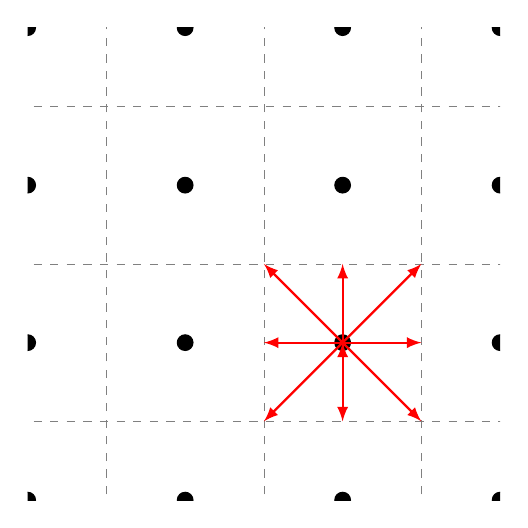
\begin{tikzpicture}
    \coordinate (Origin)   at (0,0);
    \coordinate (XAxisMin) at (-1,0);
    \coordinate (XAxisMax) at (5,0);
    \coordinate (YAxisMin) at (0,-1);
    \coordinate (YAxisMax) at (0,5);

    \clip (-1,-1) rectangle (5cm,5cm); % Clips the picture...
    \coordinate (Bone) at (0,2);
    \coordinate (Btwo) at (2,-2);
    \draw[style=help lines,dashed] (-14,-14) grid[step=2cm] (14,14);
    \foreach \x in {-7,-6,...,7}{% Two indices running over each
      \foreach \y in {-7,-6,...,7}{% node on the grid we have drawn 
        \node[draw,circle,inner sep=2pt,fill] at (1+2*\x,1+2*\y) {};
      }
    }
    \coordinate (exm)   at (3,1);
    \foreach \x in {0, 1, -1}{
    	\foreach \y in {0, 1, -1}{
		    \draw [thick,-latex,red] (exm)
			  --( $(exm) + (\x ,\y)$ ) node [] {};
	    }
    }
  \end{tikzpicture}
}
%
			\caption*{One streaming step for a D2Q9-stencil}
		\end{figure}
	}
	\only<3>{
		\begin{figure}[htbp]
			\centering
			\setlength\figureheight{0.675\textheight} 
			\setlength\figurewidth{\figureheight} 
			\resizebox{\figurewidth}{\figureheight}{
 \begin{tikzpicture}
    \coordinate (Origin)   at (0,0);
    \coordinate (XAxisMin) at (-1,0);
    \coordinate (XAxisMax) at (5,0);
    \coordinate (YAxisMin) at (0,-1);
    \coordinate (YAxisMax) at (0,5);
    \clip (-1,-1) rectangle (5cm,5cm); % Clips the picture...
    \coordinate (Bone) at (0,2);
    \coordinate (Btwo) at (2,-2);
    \draw[style=help lines,dashed] (-14,-14) grid[step=2cm] (14,14);
    \foreach \x in {-7,-6,...,7}{% Two indices running over each
      \foreach \y in {-7,-6,...,7}{% node on the grid we have drawn 
        \node[draw,circle,inner sep=2pt,fill] at (1+2*\x,1+2*\y) {};
      }
    }
    \coordinate (exm)   at (3,1);
    \foreach \x in {0, 1, -1}{
    	\foreach \y in {0, 1, -1}{
    		\coordinate (neigh)   at ($(exm) + 2*(\x ,\y)$);
		    \draw [thick,-latex,red] (neigh)
			  --( $(neigh) + (\x ,\y)$ ) node [] {};
	    }
    }
  \end{tikzpicture}
}
%
			\caption*{One streaming step for a D2Q9-stencil}
		\end{figure}
	}
	\end{columns}
	
\end{frame}
\begin{frame}{LBM - very short overview}
	%-collide(formula)-explicitness
	\begin{block} 
		\centering
		
		Collide step: application of the lattice Boltzmann equation
	\begin{align*}	
	f_i(\bm{x} + \bm{c_i}\Delta t, t + \Delta t) = f_i(\bm{x}, t) + \Omega_i(\bm{x}, t)
	\end{align*}
	\end{block}	
	\pause
	Density and velocity are given locally
	
		\begin{align*}
		\rho(\bm{x}, t) = \sum_i f_i(\bm{x},t)
		\end{align*}
		\begin{align*}
		\rho \bm{u}(\bm{x}, t) = \sum_i \bm{c_i} f_i(\bm{x},t)
		\end{align*}
		
		Source: \cite{kruger.2016}
\end{frame}
\subsection{Boundary Conditions}
\begin{frame}{Boundary Conditions : Expectations}
	\begin{block}
		
	\begin{itemize}
		\item Free-slip boundary conditions (Neumann Boundary Conditions)
		\item No-slip / UBB boundary conditions (Dirichlet boundary conditions)
	\end{itemize}
	\pause
	\centering
	Both are expected to converge with order 2 in $\Delta x$
	\end{block}
\end{frame}

\subsection{Thermal LBM}
\begin{frame}{Thermal LBM : Principle}
		\begin{center}
			\smartdiagram[circular diagram:clockwise]{
				Velocity Field, Thermal LBM, Force Field, Hydrodyn. LBM}
			
		\end{center}
\end{frame}



  { % Questions?
    \setbeamertemplate{footline}{}
    \begin{frame}[c,noframenumbering]
      \begin{center}
        Thanks for listening.\\
        {\bf Any questions?}
      \end{center}
    \end{frame}

    % References
    \section*{References}
    %TODO List all references or remove slides - I would only mention the references that are actually used for our presentation, my references are already there (Christoph)
    \begin{frame}[noframenumbering]{References}
      \printbibliography
    \end{frame}
  }
\end{document}

